\documentclass[letterpaper]{article}
\usepackage[draft]{aaai2026}
\usepackage{times}
\usepackage{helvet}
\usepackage{courier}
\usepackage[hyphens]{url}
\usepackage{graphicx}
\urlstyle{rm}
\def\UrlFont{\rm}
\usepackage{natbib}
\usepackage{caption}
\usepackage{amsmath,amssymb,booktabs}
% Tectonic/XeTeX defaults to TU; the AAAI PSNFSS families require legacy OT1.
% This selects the required Times/Helvetica/Courier fonts without changing the style.
\renewcommand{\encodingdefault}{OT1}
\fontencoding{OT1}\selectfont
\frenchspacing
\setcounter{secnumdepth}{2}
\title{Ranking Compiler Configurations with Graph and Tabular Models}
\author{Chan Chun Mun Aloycius (CCHAN041)\\
Ong Seng Kiat (ON0003AT)\\
Seth Yew Kuan Yang (SETH0011)\\
Eugene Ng Yi Sheng (N2602219H)\\
Tan Ying Xuan (TA0040AN)}
\affiliations{Full report draft, 22 October 2026}
\begin{document}
\maketitle
\begin{abstract}
Different compiler configurations can run the same computational graph at different speeds. We study how to rank them for the Google ``Fast or Slow? Predict AI Model Runtime'' competition. With training samples and primary histogram gradient boosting (HGB) settings fixed, richer configuration features improve ranking on both NLP collections in an earlier feature-bundle experiment. GraphSAGE outperforms matched-data HGB on XLA random but not XLA default. Percentile-target HGB improves three selected ensembles, including one where it is weaker alone. GNN component ablations establish no clear standalone benefit, and larger budgets do not consistently help. The final system improves on basic-feature HGB across all five audit collections and has a public Kaggle score of 0.56715, recorded in a post-deadline submission screenshot. Reused audit data limit generalisation. Our contribution is the evaluation of features, targets and complementary models, not a new learning algorithm.
\end{abstract}

\section{Introduction}
\subsection{Problem and Motivation}
Modern machine-learning workloads execute tensor computations whose performance depends partly on compiler decisions. A computational graph specifies the operations and dependencies, while a configuration specifies choices such as tensor layout or tiling. Two configurations can compute the same result yet have different execution times. Measuring every candidate is costly; a learned predictor can help order candidates so that promising ones are considered first. TPUGraphs provides graph, configuration and runtime observations for studying this problem \citep{tpugraphs}.

Using the competition's supplied data, we produce a ranking of configurations for each graph. Three questions guide the study: \emph{Do richer features help? When does graph learning help? Can ranking-aware targets improve ensembles?} These connect the representation of each configuration, the choice of model and the way predictions are combined.

\subsection{Challenges and Approach}
Three challenges guide the investigation. First, graph-only features are identical for every configuration of a graph; useful predictions therefore require information about the configuration choices and how those choices affect the graph's operations. Second, pooling into a feature vector can lose structural information, motivating graph message passing. Third, execution time varies greatly between graphs, but our task is to rank configurations within each graph. Predicting exact runtimes may therefore focus the model on differences that do not help identify faster configurations. We investigate targets based on relative rankings to better align training with this task.

We begin with a basic-feature histogram gradient boosting (HGB) baseline and test whether richer configuration-aware features improve the same learner. We then compare tabular prediction with GraphSAGE and examine input components, graph coverage, training data and targets. Finally, we combine useful predictions separately for each collection. CPU execution shaped the practical study scope, but computational efficiency is not the principal claim of this report.

\subsection{Contributions}
We provide a controlled feature-bundle comparison, collection-specific model comparisons, and evidence that percentile-target models can improve ensembles despite weaker standalone performance. Component ablations and budget studies identify limits to those improvements. The implementation and fixed reproduction recipes support these empirical contributions; HGB, GraphSAGE and ranking methods are established algorithms.

\section{Related Work and Attribution}
TPUGraphs introduces performance prediction over tensor-program graphs and compiler configurations, including challenges arising from graph scale and model generalisation \citep{tpugraphs}. Its official repository documents the input schema and baseline implementations \citep{tpudata}. We use the competition data and design our own bounded feature-extraction and training workflow around those inputs.

Histogram gradient boosting (HGB) learns nonlinear relationships from tabular features \citep{sklearn,hgbdocs}. With basic graph and configuration summaries, it provides our baseline for richer features and graph learning. GraphSAGE aggregates information from neighbouring nodes \citep{graphsage}; we test whether this use of connectivity improves ranking. XGBoost supplies regression and grouped pairwise objectives for a second tree learner \citep{xgboost,xgbrank}. Our structural signatures draw on Weisfeiler--Lehman neighbourhood refinement \citep{wl}, using bounded hashed summaries rather than reproducing the full kernel method or exact graph-isomorphism tests.

Prior solutions motivated tests of padding and ensembles \citep{vietbr}, GraphSAGE and collection-dependent ranking losses \citep{latenciaga}, and graph encodings and run-to-run variability \citep{duck}. According to the recorded provenance, competitor code, weights and predictions were not integrated. Their reported placements are not measured baselines here, and independent implementation alone does not establish novelty.

\section{Problem, Dataset and Evaluation}
\subsection{Inputs and Ranking Output}
Let $G=(V,E)$ denote a graph with operation codes and numeric node features. For candidate configuration $c_i$, the training data provide runtime $t_i>0$. A predictor returns a cost $s_i=f(G,c_i)$, and configurations are ordered by increasing $s_i$. At inference, runtimes are unknown. In Layout, configuration settings are attached to individual configurable operations. In Tile, each configuration is a single list of settings for the graph.

For configurations A, B and C with runtimes 10, 12 and 20, the correct ordering is A, B, C. Predicting A, C, B orders two pairs correctly but reverses B and C. Ranking depends on this order, not the numerical prediction scale: multiplying all costs by a positive constant leaves it unchanged.

\subsection{Dataset Organisation and Characteristics}
We model five collections separately: NLP default, NLP random, XLA default and XLA random for Layout, and XLA Tile. ``Default'' and ``random'' identify configuration-generation groupings; NLP and XLA identify source groupings rather than learning algorithms. Layout controls memory ordering, whereas Tile concerns tiling choices \citep{tpudata}. The schema supplies 18 layout fields per configurable node and 24 Tile configuration fields.

\begin{table}[t]
\centering
\begin{tabular}{@{}lrrr@{}}
\toprule
Collection & Graphs & Median $|V|$ & Max $|V|$ \\
\midrule
NLP default & 198 & 3,296 & 21,919 \\
NLP random & 207 & 3,296 & 21,919 \\
XLA default & 61 & 10,092 & 43,615 \\
XLA random & 69 & 10,449 & 43,615 \\
Tile & 5709 & 35 & 394 \\
\bottomrule
\end{tabular}
\caption{Graph counts in the official training data. Counts describe the supplied collection, not every model's training subset. Graph identities may overlap across collections.}
\label{tab:data}
\end{table}

Table~\ref{tab:data} reports the graph counts in the supplied training data, not the number of graphs used in every fit. XLA Layout graphs are substantially larger than Tile graphs: the XLA-random median is 10,449 nodes, compared with 35 for Tile. This motivates examining whether graph sampling discards useful context. The limited number of XLA graphs also makes graph-level evaluation variability important.

\subsection{Evaluation Metrics}
TPUGraphs motivates Kendall's tau by the need to preserve runtime order when searching the large Layout configuration space \citep{tpugraphs}. We use tau-b, which measures agreement between predicted and measured pair orderings while accounting for ties. It assesses which configuration is faster without penalising inaccurate runtime magnitudes when the order is correct. Scores are averaged equally across graphs. With concordant pairs $C$, discordant pairs $D$, and pairs tied only in either variable $T_t,T_s$,
\begin{equation}
\tau_b=\frac{C-D}{\sqrt{(C+D+T_t)(C+D+T_s)}}.
\end{equation}
Ties are handled using SciPy's implementation \citep{scipytau}. Without ties, the worked example gives $(2-1)/3=1/3$; a perfect ordering gives 1 and a complete reversal gives $-1$. Tau is not percentage accuracy. A value near zero indicates little net agreement in pair ordering.

For Tile, the aim is to shortlist configurations that can be measured and then choose the fastest. Following the top-$K$ evaluation rationale in TPUGraphs \citep{tpugraphs}, we measure how much slower the best candidate in the predicted top five is than the fastest available candidate. Our score is one minus this top-five regret. If $S_5$ contains the five candidates with lowest predicted cost, or all candidates when fewer than five exist, then
\begin{equation}
q(G)=1-\left(\frac{\min_{i\in S_5}t_i}{\min_i t_i}-1\right).
\end{equation}
The maximum is 1; a score of 0.98 means the best shortlisted candidate is 2\% slower than the fastest candidate in the evaluation pool. Models are compared using the same sampled configurations for each graph, so the optimum in this calculation is also restricted to that sample. These collection-level scores are distinct from the aggregate Kaggle score and are not averaged together to estimate it. Test submission inference ranks all supplied candidates.

\section{Methodology}
Starting from HGB with basic summaries, we test three extensions: richer tabular features, learning from graph connections, and training on relative rankings. Each addresses information that the baseline representation or target may miss.
\begin{figure*}[t]
\centering
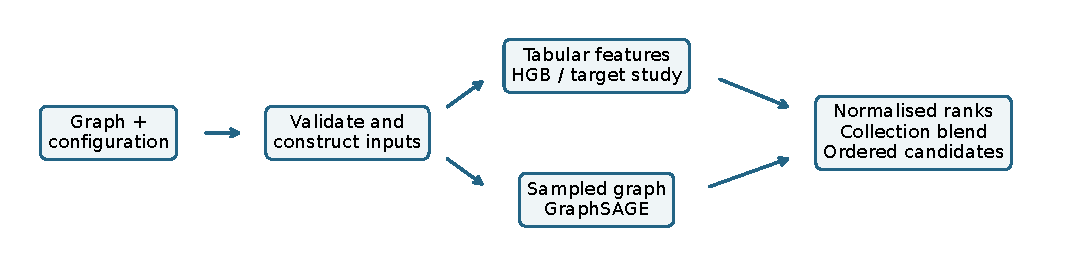
\includegraphics[width=\textwidth]{draft_assets/pipeline.pdf}
\caption{Prediction pipeline. Configuration-aware tabular models operate on all collections; GraphSAGE is evaluated and retained for XLA Layout. Model costs are converted to within-graph ranks before applying development-selected collection weights. Training labels are used only in fitting and evaluation, not feature construction.}
\label{fig:pipeline}
\end{figure*}
\subsection{Preprocessing and Sampling}
We validate array shapes, node indices and configuration values before extraction. During message passing, information flows from an operation to the operations that use its output. Numeric node features undergo a signed logarithmic transformation, $\operatorname{sign}(x)\log(1+|x|)$, after nonfinite entries are replaced with zero. Graph-level summaries are computed from these transformed features. GNN numeric inputs are additionally standardised within the sampled graph.

Configuration samples are selected independently of runtime labels and recorded by identifier. Evaluation retains at most 1,024 configurations per graph. Development splits separate graphs, so a model never trains on other configurations of its evaluation graph. Related architecture families may nevertheless occur across splits.

Layout values lie in $\{-1,0,\ldots,5\}$. We treat $-1$ as a separate invalid/default entry for feature aggregation rather than merging it with valid axis zero. Positional histograms explicitly retain that category. This handling does not claim to resolve every semantic detail of the compiler's default layout strategy. Configuration tensors are read in bounded chunks, avoiding unnecessary expansion of entire archives into memory.

\subsection{Baseline Model: Basic-Feature HGB}
\label{sec:baseline}
HGB is an ensemble of gradient-boosted decision trees. Our basic-feature HGB baseline (``Basic HGB'' in the tables) represents each graph and configuration as one row of numerical summaries. Graph features describe numeric node attributes, graph size and counts of operation types. For Layout, each configuration field is summarised across configurable operations using its mean, standard deviation, minimum and maximum. Invalid entries are replaced with zero, with their fraction recorded separately alongside the configurable-node count. Tile includes all 24 numeric configuration values and summary statistics.

These features let HGB distinguish configurations, but Layout summaries can hide which operation receives which setting. Swapping settings between two operations leaves their mean, standard deviation, minimum and maximum unchanged. The richer features below are designed to retain some of this lost information.

We fit scikit-learn HGB with squared-error regression, 180 iterations, learning rate 0.06, at most 31 leaves per tree, minimum leaf size 20 and $L_2$ regularisation 0.1. Internal early stopping is disabled. Baseline training is capped at 40 graphs per Layout collection or 160 Tile graphs and 256 configurations per graph, subject to availability. This is an implemented baseline using an established learner, not a reproduced competitor system.

The target for configuration $i$ of training graph $g$ is
\begin{equation}
y^{\log}_{gi}=\log(1+t_{gi})-\operatorname{median}_{j}\log(1+t_{gj}).
\label{eq:log}
\end{equation}
Here $n_g$ is the number of sampled configurations for graph $g$. Each graph contributes equal total training weight: rows receive weight proportional to $1/n_g$. Subtracting the median removes a graph-specific offset while preserving configuration order. Runtime gaps still affect the regression target, which motivates the percentile alternative in Section~\ref{sec:targets}. No runtime centre is needed at inference because predictions are used only for ordering.

This basic baseline measures the overall improvement of the final system. The separate controls used to compare model families and individual components are defined in Table~\ref{tab:design}.

\subsection{Engineered Feature Representations}
\label{sec:features}
We use \emph{engineered-feature HGB} to distinguish models using the richer representations below from the basic-feature baseline. Both use the same learning algorithm; the controlled feature experiment tests whether changing its inputs improves ranking. Final-system comparisons additionally change training budgets, targets and ensemble composition.
The Layout features address three weaknesses of basic summaries. First, statistics computed only from valid entries, together with valid-entry proportions, separate actual settings from invalid values. Second, category counts at each of the 18 configuration positions record which layout choices occur; axis identifiers represent categories, so their averages alone are difficult to interpret. Third, features associate layout choices with operation type, graph depth and connected operations. These associations help distinguish configurations with similar overall counts but different assignments.

Associations with operation type and depth are mapped into fixed-size hashed bins. Counts of category pairs along graph edges describe neighbouring choices without assuming that those choices are physically compatible. Together, the selected Layout features form a 1,140-dimensional vector.

For Tile, we retain all 24 raw settings and add signed-log values, products between pairs of the first eight transformed fields, and summaries of graph structure and neighbourhoods. These structural summaries are shared by all configurations of a graph. They provide context for interpreting configuration settings but cannot distinguish candidates on their own. The separate topology and Weisfeiler--Lehman-inspired features are included in the full Tile bundle, not the selected Layout bundle. The experiments evaluate feature bundles and selected components; they do not establish a separate benefit for every statistic.

\subsection{Neural and Graph Models}
\label{sec:gnn}
GraphSAGE tests whether learning from connected operations improves on tabular summaries. It combines each operation's features with information from its neighbours before producing a score for the configuration. We evaluate this ranker on the two XLA Layout collections. An earlier MLP study used a different protocol and is reported separately from these comparisons.

Node inputs contain transformed numeric features, a learned 16-dimensional representation of operation type, 18 configuration values and 18 validity indicators. Each indicator identifies whether its corresponding setting is valid. The mask ablation sets these indicators to zero when disabled, keeping the input dimensions unchanged.

An initial projection creates width-32 states. Two mean-neighbour aggregation layers apply residual updates:
\begin{align}
m_v^{(\ell)}&=\operatorname{mean}_{u\in\mathcal N^-(v)}h_u^{(\ell)},\\
h_v^{(\ell+1)}&=h_v^{(\ell)}+\operatorname{ReLU}
 \bigl(W_\ell[h_v^{(\ell)};m_v^{(\ell)}]+b_\ell\bigr).
\end{align}
Empty neighbourhoods contribute a zero message. Mean and maximum summaries are computed over all sampled nodes and separately over configurable nodes, giving four graph summaries. Optional context histograms provide additional configuration summaries. These inputs pass through a width-32 output head with ReLU and dropout 0.05 to produce one score. The context ablation zeroes the context vector without changing the head dimensions. The no-message ablation zeroes neighbour messages while retaining the layers, testing the contribution of information passed along edges.

Within a graph's configuration batch, we use a pairwise hinge loss. For pairs with $|y_i^{\log}-y_j^{\log}|>0.02$, let $a_{ij}=\operatorname{sign}(y_i^{\log}-y_j^{\log})$. Then
\begin{equation}
\mathcal L=\frac{1}{|\mathcal P|}\sum_{(i,j)\in\mathcal P}
\max\{0,0.1-a_{ij}(s_i-s_j)\}.
\end{equation}
Larger costs should correspond to slower configurations. If no pair is eligible, smooth-$L_1$ regression is used for that batch. This surrogate encourages ordering but does not optimise tau-b exactly.

\subsection{Alternative Targets and Objectives}
\label{sec:targets}
The baseline target removes each graph's median log runtime, but regression still gives weight to the sizes of runtime gaps. We test whether learning relative positions is more useful for ranking. Each training runtime is replaced by its percentile position among the sampled configurations of the same graph:
\begin{equation}
y^{\mathrm{pct}}_{gi}=\frac{\operatorname{rank}(t_{gi})-1}{\max(1,n_g-1)},
\end{equation}
using average ranks for ties. The fastest distinct sample receives 0 and the slowest 1. This equalises target ranges across training graphs and reduces the influence of extreme runtime gaps, although it also discards information about their magnitude. For runtimes 10, 12 and 20, the percentile targets are 0, 0.5 and 1. They describe position, not predicted runtime units.

To test the HGB target, we train on the same examples with the same features and tree settings, changing only the labels. Separately, we compare XGBoost regression with \texttt{rank:pairwise} while keeping its model settings fixed. Configurations are grouped by graph, with faster candidates assigned higher relevance and ties retained. We negate the ranker's output so lower scores still indicate faster configurations. Comparing HGB with XGBoost changes the learning algorithm as well as the objective, so it cannot isolate the effect of the objective alone.

\subsection{Prediction Blending}
Models may make different ranking errors, so combining them can help even when one is weaker on its own. We first convert each model's predictions to within-graph ranks $r_{mgi}/n_g$, using average ranks for ties. This puts outputs from different training targets on a common scale. Predictions are averaged over seeds and, for the final test ensemble, over the two folds. Fixed nonnegative weights for each collection then produce
\begin{equation}
S_{gi}=\sum_m w_m\overline r_{mgi},\qquad \sum_mw_m=1.
\end{equation}
Candidates are sorted by increasing $S_{gi}$. During development, each graph is scored only by models that did not train on it.

\section{Experimental Setup}
Table~\ref{tab:design} separates whole-system improvement, controlled component comparisons and ensemble selection. Each answers a different question; their gains should not be added together.

\begin{table*}[t]
\centering
\small
\begin{tabular}{@{}p{0.17\textwidth}p{0.36\textwidth}p{0.42\textwidth}@{}}
\toprule
Experiment & Comparison & What it can establish \\
\midrule
Whole system & Basic HGB versus final ensemble on the same audit graphs & Overall improvement; several pipeline choices change together. \\
Model family & GraphSAGE versus HGB with matched training data & Relative performance on common development folds. \\
Tabular features & Basic versus richer features; HGB and samples fixed & Bundle-level benefit under the earlier audit protocol. \\
GNN components & Mask/context additions; full GNN versus no messages & Effect of each change at fixed graph and training budgets. \\
Graph and data budgets & Vary graph sample size or training-data quantity & Budget sensitivity; computation also changes. \\
Training target & HGB log-runtime versus percentile; XGBoost regression versus pairwise & Target/objective effect within the same learner and samples. \\
Ensemble update & Existing system versus blends with a new model & Contribution to the combined ranking. \\
\bottomrule
\end{tabular}
\caption{Experiment design and controls. Basic HGB, matched-data HGB and the reference GNN serve different purposes. Earlier feature experiments and later development studies use different protocols.}
\label{tab:design}
\end{table*}

\subsection{Splits, Budgets and Hardware}
\label{sec:splits}
Development uses two disjoint blocks of 12 graphs per collection from official training data. A held-out graph may train the other fold, but only held-out predictions guide selection. A separate audit uses previously inspected official validation graphs: 20 per NLP collection, seven per XLA Layout collection and 24 for Tile. Thus the 24 development graphs guide selection, while the audit provides additional, reused evidence rather than an untouched test.

The final models use different amounts of training data. NLP default uses 128 graphs and 32,768 configurations per fold; NLP random uses 195 graphs and 74,880 configurations. XLA-default HGB uses 40 graphs and 10,240 configurations, while its GNN uses 49 graphs and 12,544 configurations. XLA-random models use 57 graphs, with 13,440/13,676 HGB examples and 6,864/6,972 GNN examples in folds 0/1. Tile uses 320 graphs and 64,467/64,630 examples. These are actual counts; some graphs contain fewer configurations than the sampling limit.

Training ran in CPU-based Colab sessions with approximately 12--13 GB of RAM. GPU resources were potentially available, but the team chose CPU execution because of the administrative process required to access them. Graph sampling and resumable jobs made the experiments practical; this setup was not a competition restriction or a measured efficiency advantage over GPU systems.

The larger final HGB models use 300 iterations, 63 leaves, minimum leaf size 10 and learning rate 0.04; XLA-default HGB retains the baseline settings. GNNs use AdamW with learning rate 0.001, weight decay $10^{-4}$, batch size 16 configurations, gradient clipping at 5, at most 20 epochs and patience 5. Early stopping monitors tau on up to 128 fixed development configurations per graph; final comparisons use all saved evaluation candidates. The final GNN samples contain at most 2,048 nodes for XLA default and 512 for XLA random. XGBoost screening uses 300 trees, depth 6, learning rate 0.04, histogram bins capped at 128 and four sampled pairs per example for pairwise training.

\subsection{Controlled Comparisons and Selection}
We first screen candidates using seed 42, then repeat selected comparisons with seeds 42, 137 and 2026. Screening identifies promising settings; confirmation checks their sensitivity to configuration sampling and model randomness. The graph splits remain fixed. Some deterministic HGB repetitions coincide, so three seeds do not represent three independent datasets.

To test graph coverage, we retain up to 512, 1,024, 2,048 or 4,096 nodes. Configurable nodes are capped at three quarters of that limit and edges at eight times the limit. This experiment fixes 24 training graphs and 64 configurations per graph. We then test 24, 40 or all eligible training graphs and 64, 128 or 256 configurations. These comparisons vary data quantity, but do not hold computation constant: more examples also require more training work.

For the final ensemble update, we give each new model a weight of 0.25, 0.5, 0.75 or 1.0. When GraphSAGE is already present, we also test replacing only the HGB component. We accept an update only if mean development tau improves by at least 0.002 without a decline in either fold, followed by confirmation across seeds. This avoids accepting an average gain driven by one fold. Earlier stages used their recorded selection rules; audit scores do not override rejected updates.

\subsection{Uncertainty and Evidence Scope}
Paired comparisons use the same graphs and configurations. For component intervals, we average each graph's score changes across seeds, then bootstrap by resampling graphs. The reported 95\% intervals are exploratory: they are not adjusted for testing many alternatives and do not fully account for repeatedly using the same data to guide decisions. An interval spanning zero establishes neither the direction of an effect nor its absence. Precision depends on the number of graphs and variation between them; we have not shown that a few unusual graphs explain the wide intervals. XLA default/random can share graphs, so these collections are not independent replications.

We report absolute score differences first. Relative tau improvements near a zero baseline can be misleading and are omitted for XLA default. Whole-system comparisons can change features, training data, model family and ensemble composition simultaneously; they establish the final pipeline's recorded performance but cannot identify a single causal component.

\section{Results and Discussion}
Sections~\ref{sec:feature_results}, \ref{sec:family_results} and \ref{sec:ensembles} answer the three research questions in turn. Component and budget studies explain the limits of those findings; the final comparison measures overall improvement.

\subsection{Feature Engineering with HGB Held Fixed}
\label{sec:feature_results}
Richer features improve HGB on both NLP collections in the controlled feature-bundle experiment. With training samples and primary model settings fixed, mean audit tau across seeds increases from 0.2358 to 0.3016 on NLP default and from 0.3322 to 0.4741 on NLP random. Paired gains are 0.0658 and 0.1419, with exploratory 95\% intervals [0.0430, 0.0886] and [0.1045, 0.1820]. Both intervals lie above zero.

The result supports retaining more information about layout choices and their associated operations, while keeping HGB as the learner. It establishes a benefit for the bundle, not for each feature individually. This earlier experiment uses reused audit data and differs from the final-system comparison. Confirmation on untouched graphs would strengthen the finding.

\subsection{Model-Family Comparisons}
\label{sec:family_results}
Graph learning helps on XLA random but not XLA default in the matched-data comparison. Table~\ref{tab:family} compares GraphSAGE and HGB on common development folds at seed 42. Basic HGB is shown for context, but uses a separate training budget; its final-system comparison appears in Table~\ref{tab:final}.
\begin{table}[t]
\centering
\begin{tabular}{@{}llrrr@{}}
\toprule
XLA & Model & Fold 0 & Fold 1 & Mean \\
\midrule
default & Basic HGB & 0.1324 & 0.1281 & 0.1302 \\
 & Matched HGB & 0.1218 & 0.1437 & 0.1328 \\
 & GraphSAGE & 0.0191 & 0.0594 & 0.0393 \\
random & Basic HGB & 0.3087 & 0.1455 & 0.2271 \\
 & Matched HGB & 0.3306 & 0.2703 & 0.3005 \\
 & GraphSAGE & 0.4084 & 0.3482 & 0.3783 \\
\bottomrule
\end{tabular}
\caption{Model-family screening at seed 42 on common development folds. Matched HGB shares GraphSAGE training examples/budgets; basic HGB uses its separate baseline budget. All values are Kendall tau.}
\label{tab:family}
\end{table}

On XLA random, GraphSAGE exceeds matched HGB on both folds, with mean tau 0.3783 versus 0.3005, an absolute gain of 0.0778. On XLA default, it scores 0.0393 versus 0.1328 and is weaker on both folds. The reversal matters: choosing GraphSAGE solely because the input is a graph would improve one collection while weakening the other in this comparison.

One possible explanation concerns the configurations being ranked. TPUGraphs describes default-search configurations as more similar to one another than random-search configurations \citep{tpugraphs}. GraphSAGE may capture distinctions among diverse configurations more readily than small differences among similar ones. However, these experiments do not establish that explanation: graph sampling, model capacity and the training objective may also affect the outcome. The comparison changes both architecture and representation; the message-passing ablation below asks a narrower question about the role of graph connections.

We therefore select models separately for each collection. The final XLA-default ensemble retains a GNN because its predictions can complement HGB, even though its standalone score is lower. Section~\ref{sec:ensembles} distinguishes this ensemble benefit from standalone superiority.

Earlier MLP exploration produced local ranking scores of 0.1002/0.2752 on NLP default/random and 0.1697/0.2469 on XLA default/random, with a Tile score of 0.9068. These historical values describe a different evaluation protocol and are included only to document the explored model family. They cannot be subtracted from the later HGB/GNN values as controlled improvements. Gated GraphSAGE code also exists, but no verified executed outcome was recovered; we make no measured success or failure claim for it.

\subsection{Component and Target Ablations}
We next test whether individual GNN inputs, neighbour messages or different training targets improve ranking. These comparisons use the controls in Table~\ref{tab:design}.
\begin{figure*}[t]
\centering
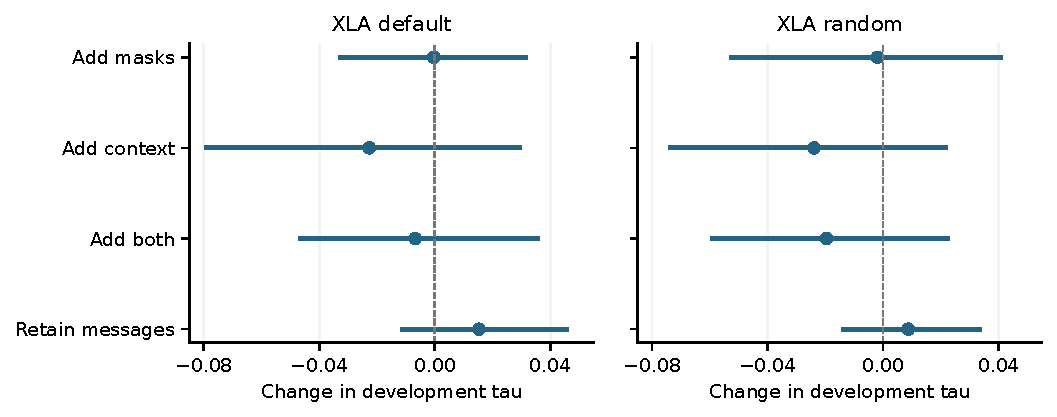
\includegraphics[width=\textwidth]{draft_assets/components.pdf}
\caption{GNN component comparisons on 24 development graphs across two folds, with three-seed confirmation. Additions compare with the same-budget reference GNN; retaining messages compares the full model with its no-message control. Dots show mean changes in tau and horizontal bars show exploratory 95\% graph-bootstrap intervals. All intervals span zero, so none establishes a clear direction of effect. These effects are not additive.}
\label{fig:components}
\end{figure*}

\subsubsection{Validity Masks and Context}
Validity masks identify usable settings, while context histograms supply configuration summaries alongside the graph representation. Figure~\ref{fig:components} tests whether either adds useful information at the chosen node budgets. Masks change development tau by $-0.0003$ on XLA default and $-0.0019$ on XLA random; context alone changes it by $-0.0227$ and $-0.0239$. Adding both changes it by $-0.0068$ and $-0.0196$. All intervals cross zero. For example, the combined-addition interval is [$-0.0465$, 0.0355] on default and [$-0.0591$, 0.0224] on random.

The combined XLA-default interval includes both losses and gains, so the direction of the effect remains uncertain. This does not show that masks and context have no effect. Including them in a selected larger-data model also does not prove a separate benefit. Unlike the HGB feature-bundle comparison, these GNN input tests do not establish a clear improvement.

\subsubsection{Message Passing}
The message-passing ablation tests whether information from connected operations helps beyond processing node features alone. Comparing the full GNN with the otherwise corresponding no-message model yields gains of 0.0153 on XLA default and 0.0088 on XLA random. The respective intervals are [$-0.0112$, 0.0457] and [$-0.0137$, 0.0334]. These positive estimates are consistent with useful structural information, but neither interval establishes a clear standalone gain. The stronger XLA-random GraphSAGE result therefore cannot be attributed solely to message passing.

\subsubsection{Target Transformation and Training Objective}
The target study asks whether predicting relative positions improves ordering even when features and training examples stay fixed. In Table~\ref{tab:targets}, percentile targets improve HGB mean development tau from 0.3874 to 0.4396 on NLP default and from 0.1288 to 0.1520 on XLA default. They slightly reduce NLP-random tau from 0.7242 to 0.7217 and reduce XLA-random tau from 0.3091 to 0.3002. Thus a target that more directly describes ranking is useful in some collections, but not all. Percentiles remove differences in target ranges and runtime-gap sizes that remain after median centring; discarding those gaps may also remove useful information. This tradeoff is a possible interpretation, not a tested causal explanation.
\begin{table}[t]
\centering
\begin{tabular}{@{}lrrrr@{}}
\toprule
Collection & H-log & H-pct & X-reg & X-pair \\
\midrule
NLP def. & 0.3874 & 0.4396 & 0.3683 & 0.4146 \\
NLP rand. & 0.7242 & 0.7217 & 0.6718 & 0.6968 \\
XLA def. & 0.1288 & 0.1520 & 0.0577 & 0.1356 \\
XLA rand. & 0.3091 & 0.3002 & 0.3280 & 0.2940 \\
\bottomrule
\end{tabular}
\caption{Mean development tau over two folds at seed 42. H-log/H-pct compare HGB targets; X-reg/X-pair compare XGBoost objectives. Training examples match within each collection. These standalone screen results differ from confirmed ensemble gains.}
\label{tab:targets}
\end{table}

Within XGBoost, pairwise ranking improves on regression for NLP default (0.3683 to 0.4146), NLP random (0.6718 to 0.6968) and XLA default (0.0577 to 0.1356), but declines on XLA random (0.3280 to 0.2940). This supports testing the objective directly rather than assuming a ranking loss must win. Neither XGBoost arm enters the final ensemble under the recorded selection rule. That outcome concerns this fixed screening configuration, not the general potential of XGBoost or pairwise methods. The final target study reuses existing GNNs and does not test a new GNN objective.

\subsection{Graph Coverage and Training-Budget Experiments}
To assess whether the mixed GNN results depend on the chosen budgets, we test larger graph samples, more training examples and longer training.
\begin{figure*}[t]
\centering
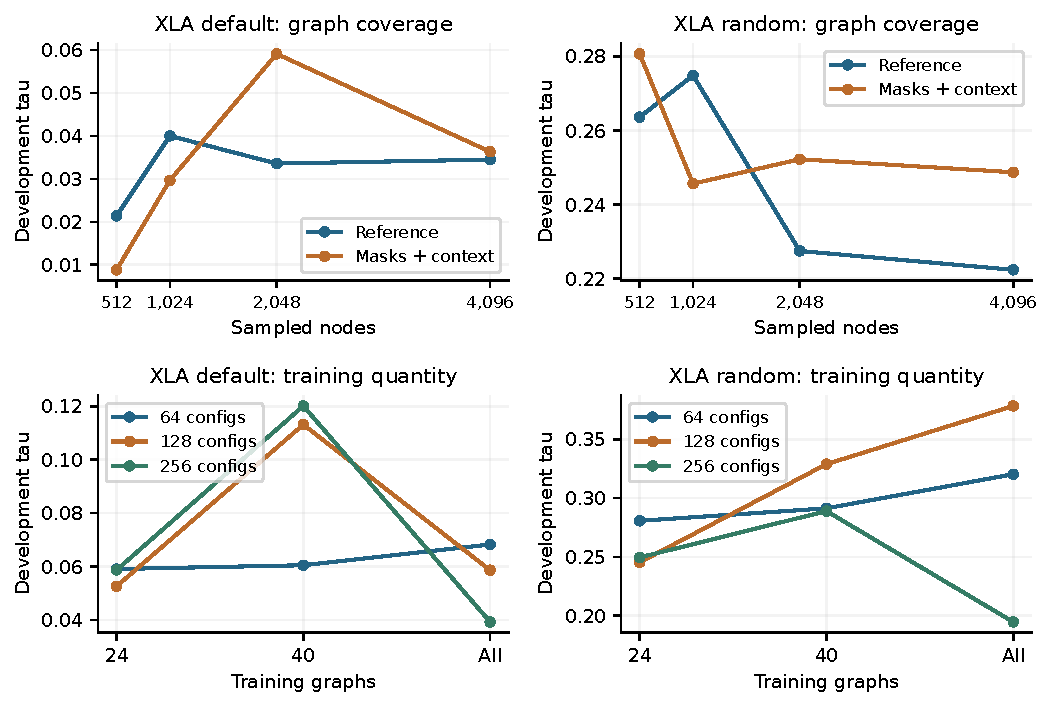
\includegraphics[width=\textwidth]{draft_assets/scaling.pdf}
\caption{Seed-42 screening, averaged over two development folds. Top: node, configurable-node and edge caps change together at fixed initial training data. Bottom: data budgets vary for the full GNN at the selected graph budget; ``all'' means all eligible training graphs in a fold. Larger budgets do not give monotonic improvements. Optimiser work changes with the number of training examples.}
\label{fig:scaling}
\end{figure*}

\subsubsection{Sampled Graph Coverage}
Retaining more of a graph does not consistently improve ranking (Figure~\ref{fig:scaling}). For the full XLA-default GNN, mean development tau rises from 0.0088 at 512 nodes to 0.0591 at 2,048, then falls to 0.0363 at 4,096. On XLA random, the 512-node model scores 0.2807, exceeding the larger samples in this screen. We therefore choose graph sample sizes separately by collection. Sampling changes both the available neighbourhoods and training demands; this experiment does not identify which explains the pattern.

\subsubsection{Training-Data Quantity}
Data scaling also produces collection-specific outcomes. For XLA random, the full GNN rises from 0.2807 at 24 graphs and 64 configurations to 0.3783 with all eligible graphs and 128 configurations. Increasing to 256 configurations at all eligible graphs lowers the screened mean to 0.1947. On XLA default, 40 graphs and 256 configurations scores 0.1201, whereas the all-eligible-graph/256 setting scores 0.0393. The final choice is based on recorded system selection rather than simply selecting the largest dataset or the highest standalone entry from this screen.

Training HGB on more data improves NLP random: development tau increases from 0.7079 to 0.7242 after confirmation, with gains in both folds. Reused-audit tau rises from 0.6466 to 0.6725, a gain of 0.0259 with interval [0.0122, 0.0426], improving 17 of 20 graphs. For NLP default, the confirmed mean development gain is 0.0084, but one fold declines by 0.0006. We reject that update because the selection rule requires neither fold to worsen, regardless of its later audit score.

For Tile, training on 640 graphs underperforms the existing model at both 256 and 384 configurations. Larger settings were not run because of resource requirements; their predictive performance is unknown.

\subsubsection{Longer Training}
Allowing up to 40 GNN epochs with patience 10 does not produce an update that meets the selection rule. On XLA default, a 50/50 blend with the longer-trained GNN gains 0.0022 on average at seed 42, but one fold worsens. The corresponding selected-weight XLA-random blend loses 0.0177, so we retain the earlier models. Saved curves show training loss and early-stopping development tau, not validation loss; they cannot establish an absence of overfitting.

\subsection{Ensemble Selection and Complementarity}
\label{sec:ensembles}
Adding percentile-target HGB improves the ensemble for three collections, so we include these models in the final combinations. Confirmed mean development gains are 0.0665 for NLP default, 0.0050 for NLP random and 0.0293 for XLA default. XLA random and Tile remain unchanged. Table~\ref{tab:recipe} gives the model weights; Section~\ref{sec:splits} records the training data used.
\begin{table}[t]
\centering
\begin{tabular}{@{}lrrr@{}}
\toprule
Collection & HGB log & HGB pct & GNN \\
\midrule
NLP default & 25\% & 75\% & -- \\
NLP random & 50\% & 50\% & -- \\
XLA default & 37.5\% & 25\% & 37.5\% \\
XLA random & 25\% & -- & 75\% \\
Tile & 100\% & -- & -- \\
\bottomrule
\end{tabular}
\caption{Final rank-blend weights. Each component averages recorded seeds and both folds for test inference. NLP random uses expanded-data HGB; GNN node budgets are 2,048 for XLA default and 512 for XLA random. No XGBoost model is selected.}
\label{tab:recipe}
\end{table}


The final system uses engineered-feature HGB in all five collections. NLP combines log-runtime and percentile-target HGB; XLA Layout also includes GraphSAGE; Tile uses log-runtime HGB alone. The ensemble combines predicted rankings rather than raw runtime estimates. XGBoost and the earlier MLP are not included. Retaining HGB does not mean retaining the basic-feature baseline: the representation, selected training settings and, where applicable, targets and blends have changed.

NLP random shows why a weaker model can still help an ensemble. Percentile HGB is slightly worse than log-runtime HGB alone in screening, yet their 50/50 combination meets the development rule and improves the audit. Models can make different mistakes, so averaging their ranks can correct some errors. This benefit is specific to the tested combination: some earlier blends improved development scores without improving the audit.

These ensemble updates also improve reused-audit tau: NLP default increases from 0.4113 to 0.4536, NLP random from 0.6725 to 0.6843, and XLA default from 0.0352 to 0.0943. Paired gains are 0.0423, 0.0118 and 0.0592, with exploratory intervals [0.0222, 0.0634], [0.0068, 0.0180] and [0.0313, 0.0927]. They improve 15/20, 18/20 and 7/7 audit graphs respectively. These small, reused samples provide supporting evidence, not an independent test of the selected ensembles.

\subsection{Final Performance}
We return to basic HGB to assess the combined effect of the selected features, models and blends.
\begin{table}[t]
\centering
\begin{tabular}{@{}lrrrr@{}}
\toprule
Collection & $n$ & Basic & Final & $\Delta$ \\
\midrule
NLP default & 20 & 0.2563 & 0.4536 & +0.1972 \\
NLP random & 20 & 0.3795 & 0.6843 & +0.3047 \\
XLA default & 7 & 0.0109 & 0.0943 & +0.0834 \\
XLA random & 7 & 0.1287 & 0.2712 & +0.1425 \\
Tile & 24 & 0.9505 & 0.9793 & +0.0288 \\
\bottomrule
\end{tabular}
\caption{Whole-system comparison on reused audit graphs. Layout rows report mean Kendall tau; Tile reports one minus top-five regret. These different metrics must not be averaged into a Kaggle score. Gains are absolute.}
\label{tab:final}
\end{table}

Table~\ref{tab:final} compares the whole selected system with the basic baseline on the same reused audit graphs. All five recorded scores improve. NLP default gains 0.1972 tau and NLP random gains 0.3047; the XLA gains are 0.0834 and 0.1425. Tile rises from 0.9505 to 0.9793 in its separate local score. These are joint pipeline improvements involving representation, data, targets and ensembles. They must not be attributed to an individual mask or summed from component ablations.

The final submitted CSV contains 894 rows and preserves the competition's ordered identifiers. Relative to the preceding 0.558 submission, 42 graph rankings changed: 17 NLP default, 17 NLP random and eight XLA default. The supplied Kaggle screenshot records a public score of \textbf{0.56715} and a private score of \textbf{0.49624} for \texttt{submission\_selected.csv}. Compared with the previously reported public score of 0.558, the public improvement is approximately 0.009; the earlier score is available only at rounded precision. Three collections changed together, so this aggregate increment cannot be assigned to one collection. Earlier rounded score descriptions are omitted from precise improvement calculations.

\begin{figure*}[t]
\centering
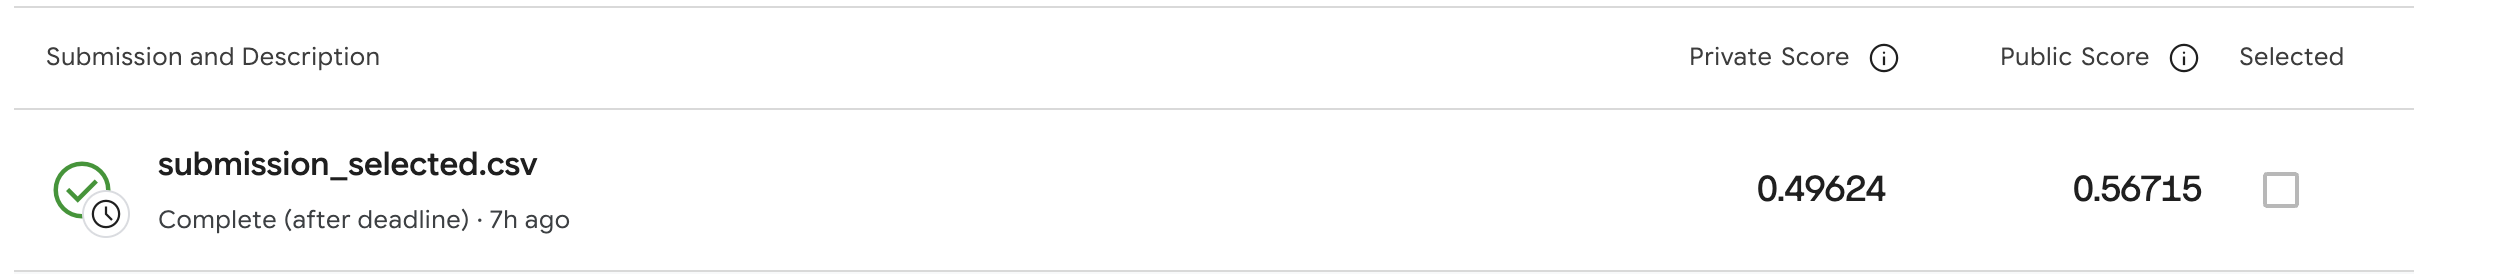
\includegraphics[width=\textwidth]{draft_assets/kaggle_submission_scores.png}
\caption{Kaggle submission record for \texttt{submission\_selected.csv}, showing a public score of 0.56715 and a private score of 0.49624. The submission is marked ``Complete (after deadline)''; the image does not establish a final leaderboard position.}
\label{fig:leaderboard}
\end{figure*}

Figure~\ref{fig:leaderboard} documents submission scores, not an official competition placement. It shows neither position nor competitor count; no relative ranking or course performance band is claimed.

\section{Limitations, Conclusion and Contributions}
\subsection{Limitations and Future Work}
The main limitation is evaluation reuse. Graph-disjoint development prevents direct within-fold graph leakage, but repeated adaptive experimentation can still fit decisions to those folds. Official validation was inspected earlier and cannot be described as untouched. The seven-graph XLA audits are particularly sensitive to individual graphs, and bootstrap intervals do not remove this limitation. Shared graph families and cross-collection identities further limit independence.

Local candidate sampling can also change the difficulty of ranking relative to full test inference. Rank-based targets describe the sampled training candidates, not an oracle ordering of every possible configuration. The practical CPU workflow constrained the architectures and data sizes examined; the results cannot rule out stronger full-graph or larger-scale GPU models. The no-gain outcomes of particular masks, context blocks and ranking objectives should therefore be read as conditional on their tested settings.

Useful future work would reserve a genuinely new graph audit, examine per-graph ensemble error correlations, and test semantic configuration features that connect axis choices to actual tensor dimensions. These are proposed investigations, not completed improvements. More training or a larger model should be justified by a specific hypothesis and matched comparisons rather than assumed to help.

\subsection{Reproducibility}
The standalone final notebook records the source implementations, graph splits, configuration identifiers and fixed recipes, including scikit-learn 1.6.1, PyTorch 2.11.0+cpu and XGBoost 3.0.5. It loads compatible models or trains missing models from raw competition data; a personal model archive is optional. The default plan contains 60 selected fits and 30 basic-baseline fits across two folds and three seeds. Optional recorded ablations expand the plan without changing the locked blend. Fresh predictions are generated by model inference rather than copied from the historical submission.

Saved notebook outputs display historical evidence in review mode; the source defaults to reproduction. Archive, split, raw-data and synthetic fitting/recovery checks validate the workflow. No full competition retraining was performed for this report, so these checks do not establish a fresh public score or guarantee identical results on other hardware. The submitted CSV remains frozen.

\subsection{Conclusion}
The main controlled finding is that richer configuration features improve HGB ranking on both NLP collections in the earlier feature-bundle experiment. GraphSAGE then provides a collection-dependent alternative, outperforming matched HGB on XLA random but not XLA default. Finally, models trained on relative rankings improve selected ensembles even when they are weaker alone. The inconclusive GNN component intervals establish neither benefit nor harm under the tested settings, and larger budgets do not consistently help. Together, these results support improving representations and selecting complementary models by collection, without requiring a new learning algorithm.

The selected system improves the recorded basic-HGB audit scores across all five collections. Its screenshot-supported public and private Kaggle scores are 0.56715 and 0.49624; the submission is marked as completed after the deadline and does not establish an official leaderboard position. Reused evaluation data limit generalisation claims, so the results support the tested pipeline rather than a universally best architecture or training target.

\subsection{Individual Contributions}
\textbf{Chan Chun Mun Aloycius} analysed the experimental results and compared model performance.

\textbf{Ong Seng Kiat} contributed to exploratory data analysis (EDA) and model implementation.

\textbf{Seth Yew Kuan Yang} drafted the report and contributed to model development and EDA.

\textbf{Eugene Ng Yi Sheng} researched candidate methods and developed the project code.

\textbf{Tan Ying Xuan} researched candidate methods and contributed to EDA.

All five members contributed equally to the project through their respective roles and participated in group calls to discuss and interpret the experimental results.

\bibliography{report_references}
\end{document}
